\documentclass{ximera}  


%\usepackage{todonotes}
%\usepackage{mathtools} %% Required for wide table Curl and Greens
%\usepackage{cuted} %% Required for wide table Curl and Greens
\newcommand{\todo}{}

\usepackage{esint} % for \oiint
\ifxake%%https://math.meta.stackexchange.com/questions/9973/how-do-you-render-a-closed-surface-double-integral
\renewcommand{\oiint}{{\large\bigcirc}\kern-1.56em\iint}
\fi


\graphicspath{
  {./}
  {jpg}
  {ximeraTutorial/}
  {basicPhilosophy/}
  {functionsOfSeveralVariables/}
  {normalVectors/}
  {lagrangeMultipliers/}
  {vectorFields/}
  {greensTheorem/}
  {shapeOfThingsToCome/}
  {dotProducts/}
  {partialDerivativesAndTheGradientVector/}
  {../productAndQuotientRules/exercises/}
  {../motionAndPathsInSpace/exercises/}
  {../normalVectors/exercisesParametricPlots/}
  {../continuityOfFunctionsOfSeveralVariables/exercises/}
  {../partialDerivativesAndTheGradientVector/exercises/}
  {../directionalDerivativeAndChainRule/exercises/}
  {../commonCoordinates/exercisesCylindricalCoordinates/}
  {../commonCoordinates/exercisesSphericalCoordinates/}
  {../greensTheorem/exercisesCurlAndLineIntegrals/}
  {../greensTheorem/exercisesDivergenceAndLineIntegrals/}
  {../shapeOfThingsToCome/exercisesDivergenceTheorem/}
  {../greensTheorem/}
  {../shapeOfThingsToCome/}
  {../separableDifferentialEquations/exercises/}
  {vectorFields/}
}

\newcommand{\mooculus}{\textsf{\textbf{MOOC}\textnormal{\textsf{ULUS}}}}

\usepackage{tkz-euclide}\usepackage{tikz}
\usepackage{tikz-cd}
\usetikzlibrary{arrows}
\tikzset{>=stealth,commutative diagrams/.cd,
  arrow style=tikz,diagrams={>=stealth}} %% cool arrow head
\tikzset{shorten <>/.style={ shorten >=#1, shorten <=#1 } } %% allows shorter vectors

\usetikzlibrary{backgrounds} %% for boxes around graphs
\usetikzlibrary{shapes,positioning}  %% Clouds and stars
\usetikzlibrary{matrix} %% for matrix
\usepgfplotslibrary{polar} %% for polar plots
\usepgfplotslibrary{fillbetween} %% to shade area between curves in TikZ
\usetkzobj{all}
\usepackage[makeroom]{cancel} %% for strike outs
%\usepackage{mathtools} %% for pretty underbrace % Breaks Ximera
%\usepackage{multicol}
\usepackage{pgffor} %% required for integral for loops



%% http://tex.stackexchange.com/questions/66490/drawing-a-tikz-arc-specifying-the-center
%% Draws beach ball
\tikzset{pics/carc/.style args={#1:#2:#3}{code={\draw[pic actions] (#1:#3) arc(#1:#2:#3);}}}



\usepackage{array}
\setlength{\extrarowheight}{+.1cm}
\newdimen\digitwidth
\settowidth\digitwidth{9}
\def\divrule#1#2{
\noalign{\moveright#1\digitwidth
\vbox{\hrule width#2\digitwidth}}}





\newcommand{\RR}{\mathbb R}
\newcommand{\R}{\mathbb R}
\newcommand{\N}{\mathbb N}
\newcommand{\Z}{\mathbb Z}

\newcommand{\sagemath}{\textsf{SageMath}}


%\renewcommand{\d}{\,d\!}
\renewcommand{\d}{\mathop{}\!d}
\newcommand{\dd}[2][]{\frac{\d #1}{\d #2}}
\newcommand{\pp}[2][]{\frac{\partial #1}{\partial #2}}
\renewcommand{\l}{\ell}
\newcommand{\ddx}{\frac{d}{\d x}}

\newcommand{\zeroOverZero}{\ensuremath{\boldsymbol{\tfrac{0}{0}}}}
\newcommand{\inftyOverInfty}{\ensuremath{\boldsymbol{\tfrac{\infty}{\infty}}}}
\newcommand{\zeroOverInfty}{\ensuremath{\boldsymbol{\tfrac{0}{\infty}}}}
\newcommand{\zeroTimesInfty}{\ensuremath{\small\boldsymbol{0\cdot \infty}}}
\newcommand{\inftyMinusInfty}{\ensuremath{\small\boldsymbol{\infty - \infty}}}
\newcommand{\oneToInfty}{\ensuremath{\boldsymbol{1^\infty}}}
\newcommand{\zeroToZero}{\ensuremath{\boldsymbol{0^0}}}
\newcommand{\inftyToZero}{\ensuremath{\boldsymbol{\infty^0}}}



\newcommand{\numOverZero}{\ensuremath{\boldsymbol{\tfrac{\#}{0}}}}
\newcommand{\dfn}{\textbf}
%\newcommand{\unit}{\,\mathrm}
\newcommand{\unit}{\mathop{}\!\mathrm}
\newcommand{\eval}[1]{\bigg[ #1 \bigg]}
\newcommand{\seq}[1]{\left( #1 \right)}
\renewcommand{\epsilon}{\varepsilon}
\renewcommand{\phi}{\varphi}


\renewcommand{\iff}{\Leftrightarrow}

\DeclareMathOperator{\arccot}{arccot}
\DeclareMathOperator{\arcsec}{arcsec}
\DeclareMathOperator{\arccsc}{arccsc}
\DeclareMathOperator{\si}{Si}
\DeclareMathOperator{\scal}{scal}
\DeclareMathOperator{\sign}{sign}


%% \newcommand{\tightoverset}[2]{% for arrow vec
%%   \mathop{#2}\limits^{\vbox to -.5ex{\kern-0.75ex\hbox{$#1$}\vss}}}
\newcommand{\arrowvec}[1]{{\overset{\rightharpoonup}{#1}}}
%\renewcommand{\vec}[1]{\arrowvec{\mathbf{#1}}}
\renewcommand{\vec}[1]{{\overset{\boldsymbol{\rightharpoonup}}{\mathbf{#1}}}\hspace{0in}}

\newcommand{\point}[1]{\left(#1\right)} %this allows \vector{ to be changed to \vector{ with a quick find and replace
\newcommand{\pt}[1]{\mathbf{#1}} %this allows \vec{ to be changed to \vec{ with a quick find and replace
\newcommand{\Lim}[2]{\lim_{\point{#1} \to \point{#2}}} %Bart, I changed this to point since I want to use it.  It runs through both of the exercise and exerciseE files in limits section, which is why it was in each document to start with.

\DeclareMathOperator{\proj}{\mathbf{proj}}
\newcommand{\veci}{{\boldsymbol{\hat{\imath}}}}
\newcommand{\vecj}{{\boldsymbol{\hat{\jmath}}}}
\newcommand{\veck}{{\boldsymbol{\hat{k}}}}
\newcommand{\vecl}{\vec{\boldsymbol{\l}}}
\newcommand{\uvec}[1]{\mathbf{\hat{#1}}}
\newcommand{\utan}{\mathbf{\hat{t}}}
\newcommand{\unormal}{\mathbf{\hat{n}}}
\newcommand{\ubinormal}{\mathbf{\hat{b}}}

\newcommand{\dotp}{\bullet}
\newcommand{\cross}{\boldsymbol\times}
\newcommand{\grad}{\boldsymbol\nabla}
\newcommand{\divergence}{\grad\dotp}
\newcommand{\curl}{\grad\cross}
%\DeclareMathOperator{\divergence}{divergence}
%\DeclareMathOperator{\curl}[1]{\grad\cross #1}
\newcommand{\lto}{\mathop{\longrightarrow\,}\limits}

\renewcommand{\bar}{\overline}

\colorlet{textColor}{black}
\colorlet{background}{white}
\colorlet{penColor}{blue!50!black} % Color of a curve in a plot
\colorlet{penColor2}{red!50!black}% Color of a curve in a plot
\colorlet{penColor3}{red!50!blue} % Color of a curve in a plot
\colorlet{penColor4}{green!50!black} % Color of a curve in a plot
\colorlet{penColor5}{orange!80!black} % Color of a curve in a plot
\colorlet{penColor6}{yellow!70!black} % Color of a curve in a plot
\colorlet{fill1}{penColor!20} % Color of fill in a plot
\colorlet{fill2}{penColor2!20} % Color of fill in a plot
\colorlet{fillp}{fill1} % Color of positive area
\colorlet{filln}{penColor2!20} % Color of negative area
\colorlet{fill3}{penColor3!20} % Fill
\colorlet{fill4}{penColor4!20} % Fill
\colorlet{fill5}{penColor5!20} % Fill
\colorlet{gridColor}{gray!50} % Color of grid in a plot

\newcommand{\surfaceColor}{violet}
\newcommand{\surfaceColorTwo}{redyellow}
\newcommand{\sliceColor}{greenyellow}




\pgfmathdeclarefunction{gauss}{2}{% gives gaussian
  \pgfmathparse{1/(#2*sqrt(2*pi))*exp(-((x-#1)^2)/(2*#2^2))}%
}


%%%%%%%%%%%%%
%% Vectors
%%%%%%%%%%%%%

%% Simple horiz vectors
\renewcommand{\vector}[1]{\left\langle #1\right\rangle}


%% %% Complex Horiz Vectors with angle brackets
%% \makeatletter
%% \renewcommand{\vector}[2][ , ]{\left\langle%
%%   \def\nextitem{\def\nextitem{#1}}%
%%   \@for \el:=#2\do{\nextitem\el}\right\rangle%
%% }
%% \makeatother

%% %% Vertical Vectors
%% \def\vector#1{\begin{bmatrix}\vecListA#1,,\end{bmatrix}}
%% \def\vecListA#1,{\if,#1,\else #1\cr \expandafter \vecListA \fi}

%%%%%%%%%%%%%
%% End of vectors
%%%%%%%%%%%%%

%\newcommand{\fullwidth}{}
%\newcommand{\normalwidth}{}



%% makes a snazzy t-chart for evaluating functions
%\newenvironment{tchart}{\rowcolors{2}{}{background!90!textColor}\array}{\endarray}

%%This is to help with formatting on future title pages.
\newenvironment{sectionOutcomes}{}{}



%% Flowchart stuff
%\tikzstyle{startstop} = [rectangle, rounded corners, minimum width=3cm, minimum height=1cm,text centered, draw=black]
%\tikzstyle{question} = [rectangle, minimum width=3cm, minimum height=1cm, text centered, draw=black]
%\tikzstyle{decision} = [trapezium, trapezium left angle=70, trapezium right angle=110, minimum width=3cm, minimum height=1cm, text centered, draw=black]
%\tikzstyle{question} = [rectangle, rounded corners, minimum width=3cm, minimum height=1cm,text centered, draw=black]
%\tikzstyle{process} = [rectangle, minimum width=3cm, minimum height=1cm, text centered, draw=black]
%\tikzstyle{decision} = [trapezium, trapezium left angle=70, trapezium right angle=110, minimum width=3cm, minimum height=1cm, text centered, draw=black]




 
\title{Wave Equation} 
\author{Milica Markovic} 
\outcome{Recognize and explain transmission line equivalent circuit model. Derive the equations for voltage and current waves on a transmission line from the equivalent circuit model.}
\begin{document}  
\begin{abstract}  

\end{abstract}  
\maketitle    




\section{ Wave equation on a transmission line}\label{telegrapher}

In this section, we will derive the expression for voltage and current
on a transmission line. This expression will have two variables, time $t$, and space $z$. 
So far, we have only seen voltages and currents as a function of time, because all circuit elements seen so far are lumped elements. In distributed systems,
we want to derive the equations for voltage and current for the case when the transmission
line is longer than the fraction of a wavelength.  To make sure that we
do not encounter any transmission line effects to start with, we can
look at the piece of a transmission line that is much smaller than
the fraction of a wavelength. In other words, we cut the transmission
line into small pieces to make sure there are no transmission line
effects, as the pieces are shorter than the fraction of a wavelength. We then represent each piece with
an equivalent circuit, as shown in Figure \ref{lineeqc} (a). 
To derive expressions for current and voltage on the transmission line, we will use the following five-step plan

\begin{enumerate}
\item Look at an infinitesimal length of a transmission line $\Delta z$.  

\item Represent that piece with an equivalent circuit. 

\item Write KCL, KVL for the piece in the time domain (we get
differential equations)

\item Apply phasors (equations become linear)

\item Solve the linear system of equations to get the expression for
the voltage and current on the transmission line as a function of $z$.

\end{enumerate}


Look at a small piece of a transmission line and represented it with an equivalent circuit. What is
modeled by the circuit elements?



\begin{figure}[htbp]
\begin{center}
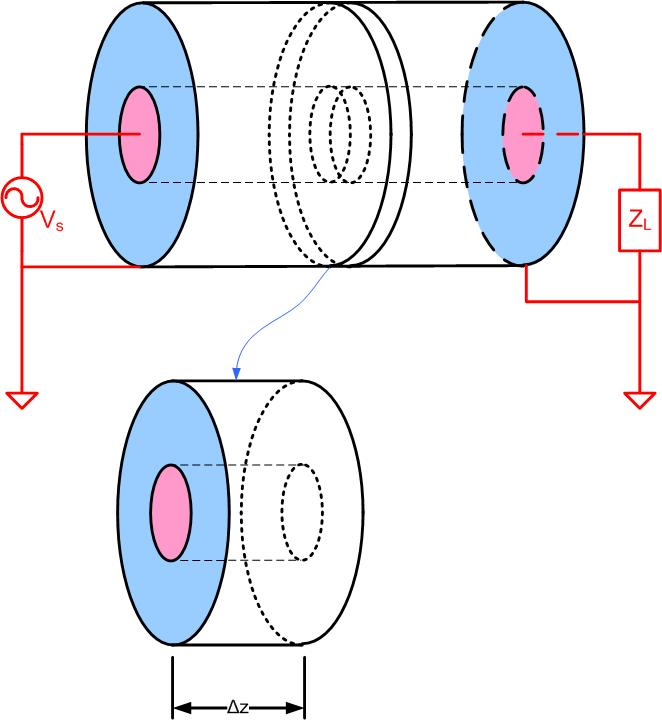
\includegraphics[scale=0.3]{../jpg/Coaxtl.jpg}
\caption{Coaxial cable is cut in short pieces.}
\label{lineeqcPieces}
\end{center}
\end{figure}

\begin{figure}[htbp]
\begin{center}
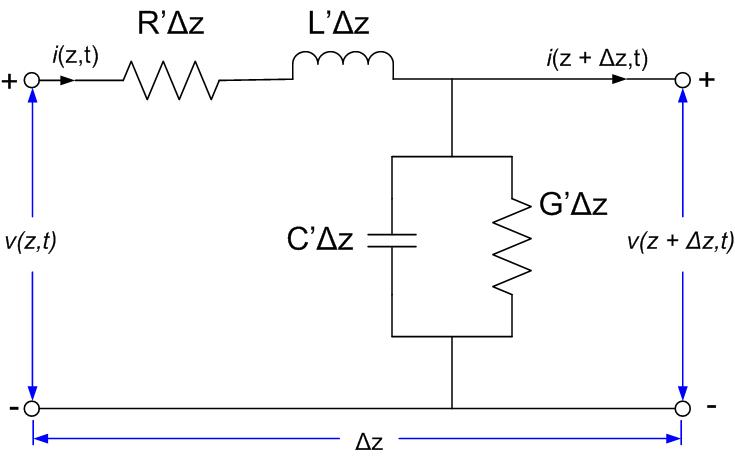
\includegraphics[scale=0.3]{../jpg/Equivalent_Circuit_of_Transmission_Line.jpg}
\caption{Equivalent circuit of a section of transmission line.}
\label{lineeqcOnePiece}
\end{center}
\end{figure}

\begin{figure}[htbp]
\begin{center}
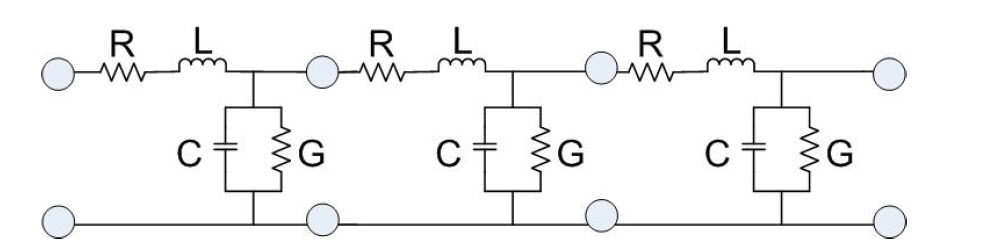
\includegraphics[scale=0.4]{../jpg/tlmadeupofcircuits.jpg}
\end{center}
\caption{Equivalent circuit of transmission line.}
\label{lineeqc}
\end{figure}



Write  KVL and KCL equations for the circuit above.

KVL
\begin{eqnarray}
-v(z,t) + R \, \Delta z \, i(z,t) + L \,\Delta z \,\frac{\partial
 i(z,t)}{\partial t} + v(z+ \Delta z,t) = 0 \nonumber
\end{eqnarray}

KCL

\begin{eqnarray}
i(z,t)=i(z+\Delta z)+ i_{CG}(z+\Delta z,t) \nonumber   \\
i(z,t)=i(z+\Delta z)+ G \, \Delta z\, v(z+\Delta z,t)+C\, \Delta z
\frac{\partial v(z+\Delta z,t)}{\partial t} \nonumber
\end{eqnarray}


Rearrange the KCL and KVL Equations \ref{te1kvl1}, \ref{te1kc11} and divide them with
$\Delta z$.  Equations \ref{te2kvl1}, \ref{te1kc21}.
let $\Delta z \to 0$ and recognize the definition of the
derivative Equations, \ref{te2kvl111}, \ref{te1kc211}.

KVL
\begin{eqnarray}
-( v(z+ \Delta z ,t)- v(z,t))=R \, \Delta z  \, i(z,t)+L  \,  \Delta z
 \frac{\partial i(z,t)}{\partial t} \label{te1kvl1}  \\ 
 -\frac{ v(z+ \Delta z ,t)- v(z,t)}{\Delta z}=R  \, i(z,t)+L  \, 
 \frac{\partial i(z,t)}{\partial t}  \label{te2kvl1} \\
\lim_{\Delta z \to 0} \{ -\frac{ v(z+ \Delta z ,t)- v(z,t)}{\Delta z}\}=  \lim_{\Delta z \to 0} \{   R  \,  i(z,t)+L  \, 
 \frac{\partial i(z,t)}{\partial t} \} \label{te2kvl111} \\
-\frac{v(z,t) }{\partial z}=R i(z,t)+L 
 \frac{\partial i(z,t)}{\partial t} \label{te3kvl1}
\end{eqnarray}

KCL

\begin{eqnarray}
-( i(z+ \Delta z ,t)- i(z,t))= G  \, \Delta z  \, v(z+\Delta z,t)+ C \, \Delta z
\frac{\partial v(z+\Delta z,t)}{\partial t} \label{te1kc11} \\
-\frac{ i(z+ \Delta z ,t)- i(z,t)}{\Delta z}= G  \, v(z+\Delta z,t)+C \, 
\frac{\partial v(z+\Delta z,t)}{\partial t} \label{te1kc21} \\
\lim_{\Delta z \to 0} \{-\frac{ i(z+ \Delta z ,t)- i(z,t)}{\Delta z} \}= \lim_{\Delta z \to 0} \{ G  \, v(z+\Delta z,t)+C \, 
\frac{\partial v(z+\Delta z,t)}{\partial t} \} \label{te1kc211} \\
-\frac{i(z,t) }{\partial z}= G  \, v(z+\Delta z,t)+C \, 
\frac{\partial v(z+\Delta z,t)}{\partial t} \label{te1kc31}
\end{eqnarray}



We just derived Telegrapher's equations in time-domain:



\begin{eqnarray}
-\frac{v(z,t) }{\partial z}=R  \, i(z,t)+L  \, 
 \frac{\partial i(z,t)}{\partial t} \nonumber  \\ \nonumber
-\frac{i(z,t) }{\partial z}= G \,  v(z+\Delta z,t)+C \, 
\frac{\partial v(z+\Delta z,t)}{\partial t} 
\end{eqnarray}


Telegrapher's equations are two differential equations with two unknowns, $i(z, t)$, $v(z, t)$. It is not
impossible to solve them; however, we would prefer to have linear algebraic equations. We then express time-domain variables as phasors.

\begin{eqnarray}
v(z,t)=Re\{ \tilde{V}(z) e^{j \omega t} \} \nonumber \\
i(z,t)=Re\{ \tilde{I}(z) e^{j \omega t} \} \nonumber
\end{eqnarray}

 $\tilde{V}(z),\tilde{I}(z) $ are the voltage, and current anywhere on the line, and they depend on the position on the line $z$. The Telegrapher's equations in phasor form are


\begin{eqnarray}
-\frac{\partial \tilde{V}(z)}{\partial z} = (R+j\omega L) \tilde{I}(z) \label{te11}\\
-\frac{\partial \tilde{I}(z)}{\partial z} = (G+j\omega C) \tilde{V}(z) \label{te121}
\end{eqnarray}



Two equations, two unknowns. To solve these equations, we first
take a derivative of both equations with respect to z. 

\begin{eqnarray}
-\frac{\partial^2 \tilde{V}(z)}{\partial z^2}=  (R+j\omega L) \frac{\partial
 \tilde{I}(z)}{\partial z}  \label{teleg3} \\
-\frac{\partial^2 \tilde{I}(z)}{\partial z^2}=  (G+j\omega C) \frac{\partial
 \tilde{V}(z)}{\partial z} \label{teleg4}
\end{eqnarray}

Rearange the previous equations:



\begin{eqnarray}
- \frac{1}{ (R+j\omega L)} \frac{\partial \tilde{I}(z)}{\partial z}= \frac{\partial^2
  \tilde{V}(z)}{\partial z^2} \label{te51} \\
-\frac{1}{ (G+j\omega C)} \frac{\partial \tilde{V}(z)}{\partial z}= \frac{\partial^2
  \tilde{I}(z)}{\partial z^2} \label{te61}
\end{eqnarray}

Substitute  Eq.\ref{te51} into  Eq.\ref{te121}
and Eq.\ref{te61} into Eq.\ref{te11} and we get

\begin{eqnarray}
-\frac{\partial^2 \tilde{V}(z)}{\partial z^2}=(G+j\omega C)(R+j\omega L) \tilde{V}(z) \label{teleg1} \\
-\frac{\partial^2 \tilde{I}(z)}{\partial z^2}= (G+j\omega C)  (R+j\omega L) \label{teleg2}
\tilde{I}(z) 
\end{eqnarray}

Or if we rearrange


\begin{eqnarray}
\frac{\partial^2 \tilde{V}(z)}{\partial z^2} -(G+j\omega C)(R+j\omega L)
 \tilde{V}(z)=0  \label{we11} \\ 
\frac{\partial^2 I(z)}{\partial z^2}- (G+j\omega C)  (R+j\omega L)
I(z)=0 \label{we21}
\end{eqnarray}

The above Equations \ref{we11}-\ref{we21} are called wave equations, and they represent
current and voltage wave on a transmission line. 
 $\gamma^2=(G+j\omega
C)(R+j\omega L)$ is the complex propagation constant. This constant
has a real and an imaginary part.

\begin{eqnarray}
\gamma= \alpha + j \beta \nonumber
\end{eqnarray}

where $\alpha$ is the attenuation constant and $\beta$ is the phase
constant.

\begin{eqnarray}
\alpha=Re\{ \sqrt{(G+j\omega C)  (R+j\omega L)  }  \} \nonumber \\ \nonumber
\beta = Im\{ \sqrt{(G+j\omega C)  (R+j\omega L)  }  \}
\end{eqnarray}

We can now write wave equations as:


\begin{eqnarray}
\frac{\partial^2 \tilde{V}(z)}{\partial z^2} -\gamma^2
 \tilde{V}(z)=0  \label{eq:TLwe11} \\ 
\frac{\partial^2 I(z)}{\partial z^2}- \gamma^2
I(z)=0 \label{eq:TLwe21}
\end{eqnarray}


The general solution of the second order differential equations with constant coefficients
Equations \ref{eq:TLwe11} - \ref{eq:TLwe21}   is:

\begin{eqnarray}
\tilde{V}(z)=\tilde{V}_0^+ e^{-\gamma z} + \tilde{V}_0^- e^{\gamma z} \nonumber \\ \nonumber
\tilde{I}(z)=\tilde{I}_0^+ e^{-\gamma z} + \tilde{I}_0^- e^{\gamma z}
\end{eqnarray}

Where $\tilde{V}(z)^+=\tilde{V}_0^+ e^{-\gamma z}$ represents the forward-going voltage wave, $\tilde{V}(z)^-=\tilde{V}_0^- e^{\gamma z}$ represents the reflected voltage wave, $\tilde{I}(z)^+=\tilde{I}_0^+ e^{-\gamma z}$ represents the forward going current wave, and $\tilde{I}(z)^-=\tilde{I}_0^- e^{\gamma z}$ represents the reflected current wave. We will see later that $\tilde{V}_0^+$ is the forward-going voltage wave at the load, $\tilde{V}_0^-$ 
is the reflected voltage wave at the load, $\tilde{I}_0^+$ is the forward going current at the load, and $\tilde{I}_0^-$ reflected current at the load.


In the next several sections, we will look at how to find the constants $\beta$, $\tilde{V}_0^+  $, $ \tilde{V}_0^-$, $\tilde{I}_0^+ $, $\tilde{I}_0^-$. In order to find the constants, we will introduce the concepts of transmission line impedance $Z_0$, reflection coefficient $\Gamma(z)$, input impedance $Z_{in}$. 


\end{document} 
